\chapter{Formal Analysis using Alloy}
This chapter presents formal analysis of the model using Alloy. The goal is to describe and correctness proof of only the most important parts of the system. 

\section{Alloy model}
\lstset{postbreak=\llap{\scriptsize\textcolor{blue}{$\hookrightarrow$}\kern0.25em}}
\lstinputlisting[language=alloy]{alloy/model.als}


\section{Generated worlds}
In order to manage the great number of different signatures, different constraints for world instances generation were proposed. Each of the instances presented below depicts a world focused on specific facts and signatures. To preserve readability, the atoms related to enumeration types were removed from the figures.

\begin{figure}[H]
    \centering
    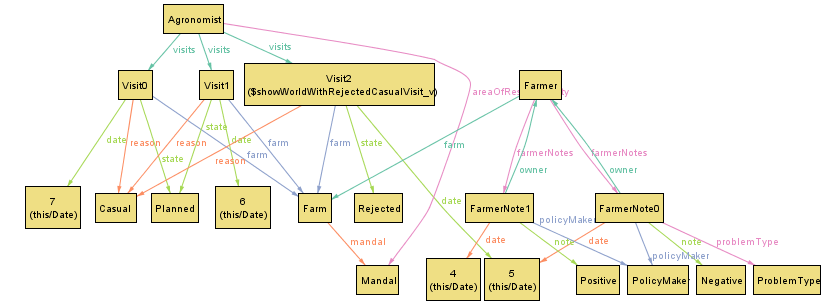
\includegraphics[width=\textwidth, keepaspectratio, origin=c]{alloy/world_instances/showWorldWithRejectedCasualVisit2.png}
    \caption{World instance focused on visits - rejected, causal visit}
    \label{fig:rejected_causal}
\end{figure}
 The first instance of worlds presented on Figure \ref{fig:rejected_causal} shows that as stated in \textbf{R63} if a casual visit is rejected, then a new casual visit is planned.
 
\begin{figure}[H]
    \centering
    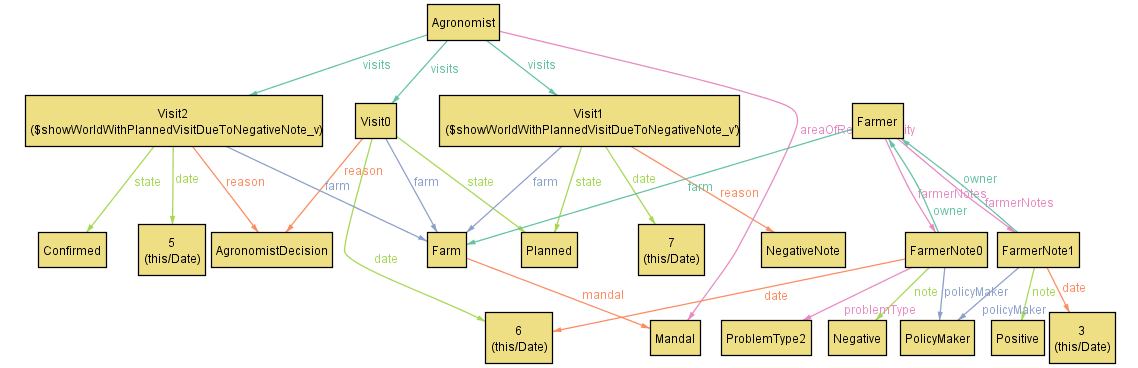
\includegraphics[width=\textwidth, keepaspectratio, origin=c]{alloy/world_instances/showWorldWithPlannedVisitDueToNegativeNote2.png}
    \caption{World instance focused on visits - planned, due to negative note visit}
    \label{fig:planned_negative_note}
\end{figure}
The world instance presented in \ref{fig:planned_negative_note} shows usage of the fact \textit{NoVisitDueToNegativeNoteIsPlannedBeforeTheDateOfTheLastNegativeNote} as the visit due to negative note is planned on date = 7 whilst the negative note was given on date = 6. Another requirement fulfilment that can be noticed is that  only a visit on or after the current day can be confirmed. The aforementioned requirement is exemplified with the date of the \textit{Visit2} (date = 5, according to the alloy script in the previous section the currentDay = 5).

\begin{figure}[H]
    \centering
    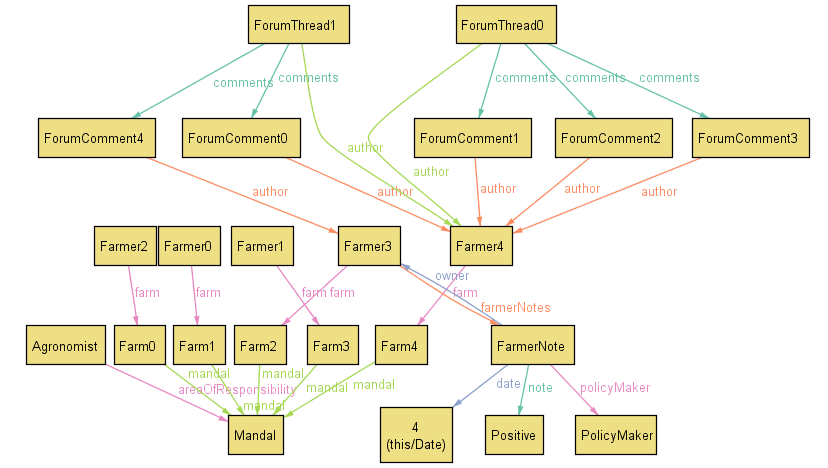
\includegraphics[width=\textwidth, keepaspectratio, origin=c]{alloy/world_instances/showWorldFocusedOnForum2.png}
    \caption{World instance focused on farmer's forum}
    \label{fig:forum}
\end{figure}
The third world instance (\ref{fig:forum}) shows many atoms related to farmer's forum. Two forum threads are created by two different farmers and some comments are added. In addition, as requirements state, each farmer possesses exactly one farm that belongs to exactly one mandal. 


\begin{figure}[H]
    \centering
    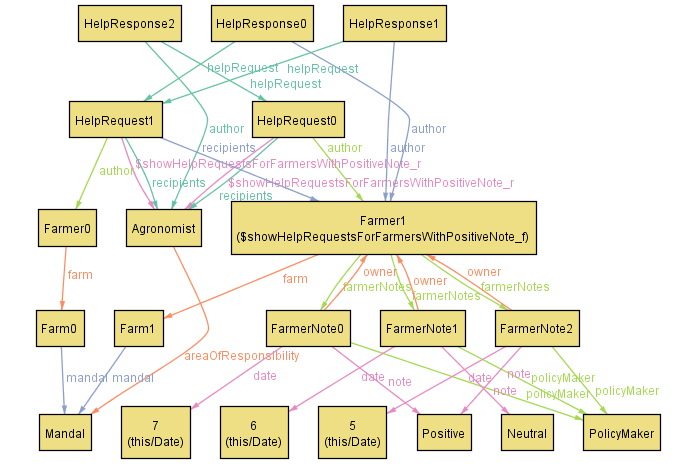
\includegraphics[width=\textwidth, keepaspectratio, origin=c]{alloy/world_instances/showHelpRequestsForFarmersWithPositiveNote2.png}
    \caption{World instance focused on help requests}
    \label{fig:help_requests}
\end{figure}
The fourth world instance (\ref{fig:help_requests}) focuses on help requests and responses. First, both help requests are obtained by an agronomist that takes care of the same mandal (the mandal is inside the agronomist's area of responsibility) as the farmers' farm who created the request. Secondly, the \textit{Farmer1} who created help responses is a farmer with positive note as stated in R35.


\begin{figure}[H]
    \centering
    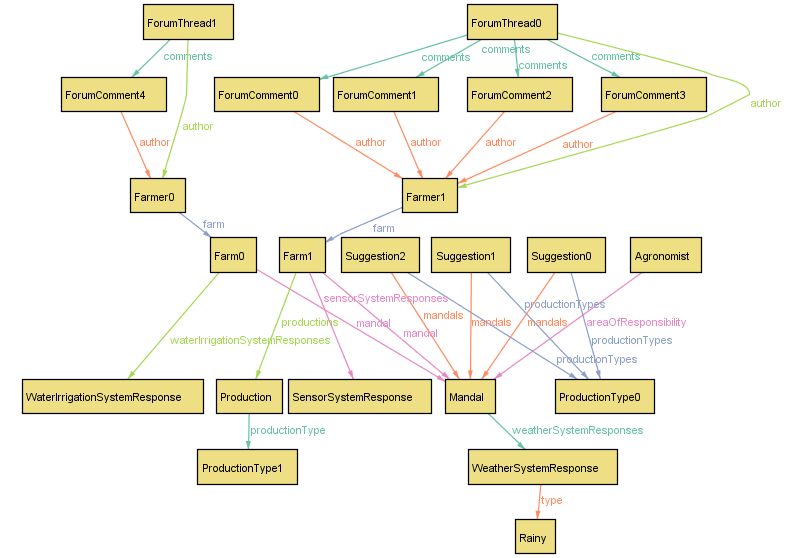
\includegraphics[width=\textwidth, keepaspectratio, origin=c]{alloy/world_instances/General2.png}
    \caption{World instance without visits (focus shifted to other atoms)}
    \label{fig:general_world}
\end{figure}
The last figure presents an instance created with the least number of constraints. It contains some types that were not presented on previous figures for clarity. For instance, atoms presenting the production of \textit{Farm1} are depicted.